\section{Background}

Bacterial biofilms are microscopic deposition of organisms that embed themselves on immersed surfaces whenever environmental conditions can sustain microbial growth.
These bacteria, when sessile, surround themselves in a self-produced viscous layer of extracellular polymeric substances.
As a result of this, the cells are extraordinarily resistant to mechanical washout or antibiotic attacks.
Most bacterial populations live in communities withing the extracellular polymeric substances.
They can be found in many different aspects of life in both positive ways (wastewater treatments, soil remediation, and groundwater protection) and negative ways (bacterial infections, dental plaque, biocorrosion of facilities and water pipes).

The recent field of energy biotechonology has lead to researching biofilms as a potential means of using plant biomass to generate sustainable fuels. %!% Recent energy biotechnolgy paper that discuss viablilty of plant biomass
\textit{Clostridium Thermocellum} is a possible choice for achieving large scale biomass conversion. %!% according to who?
Because of this there has been a surge of studies based around its behaviours and characteristics.
An interesting feature of \textit{C. Thermocellum} is that is grows as a thin cellulolytic monolayer and does not produce any extracellular polymeric matrix \citep{dumitrache2013formFunction}.
This is a stark contrast to typical biofilms which are notorious for forming complex mushroom or pillar shaped morphologies.

\cite{dumitrache2014understanding} have made a number of \textit{in situ} and \textit{in vitro} observations for \textit{C. Thermocellum}.
Here they linked the cellulose consumption rate of the bacteria to the rate of $CO_2$ produced.
The experiments ran in a continuous-flow reactor that used cellulose paper sheets innoculated with \textit{C. Thermocellum} strains.
The bacteria consumed the fibers of the cellulose sheets as they grew.
By tracking only the $CO_2$ production, they were only focused on the activity of the bacteria at a reactor-scale.
The smaller spatial movements of the bacteria were ignored for simplicity of the experiment.

Originally, biofilm models were poised as ordinary differential equations or one-dimensional partial differential equations that assumed the biofilms developed as a flat layer.
This simplified the calculation for the speed of propagation but was limited in non-spatially heterogenous biofilm morphologies. %!% Source of an old paper would suffice
To this end, many models for spatially heterogenouse biofilms were proposed.
These included stochastic individual based models, cellular automata models, and deterministic continuum models. %!% Can get a source on each
The added complexity helped in modelling more of the multi-dimensional aspects of biofilms, namely the intrinsic structures that most biofilms grew.
These models considered the changes the biofilms made at the meso-scale instead of the reactor-scale which simpler models tended to do.
The reactor-scale models attributed the spatial effects by using logistic-like growth terms to limit the amount of bacteria activity in the models. %!% Hermann paper
%!%Models have been around since the 1970s and 1980s.


\begin{figure}[h!tbp]
  \centering
  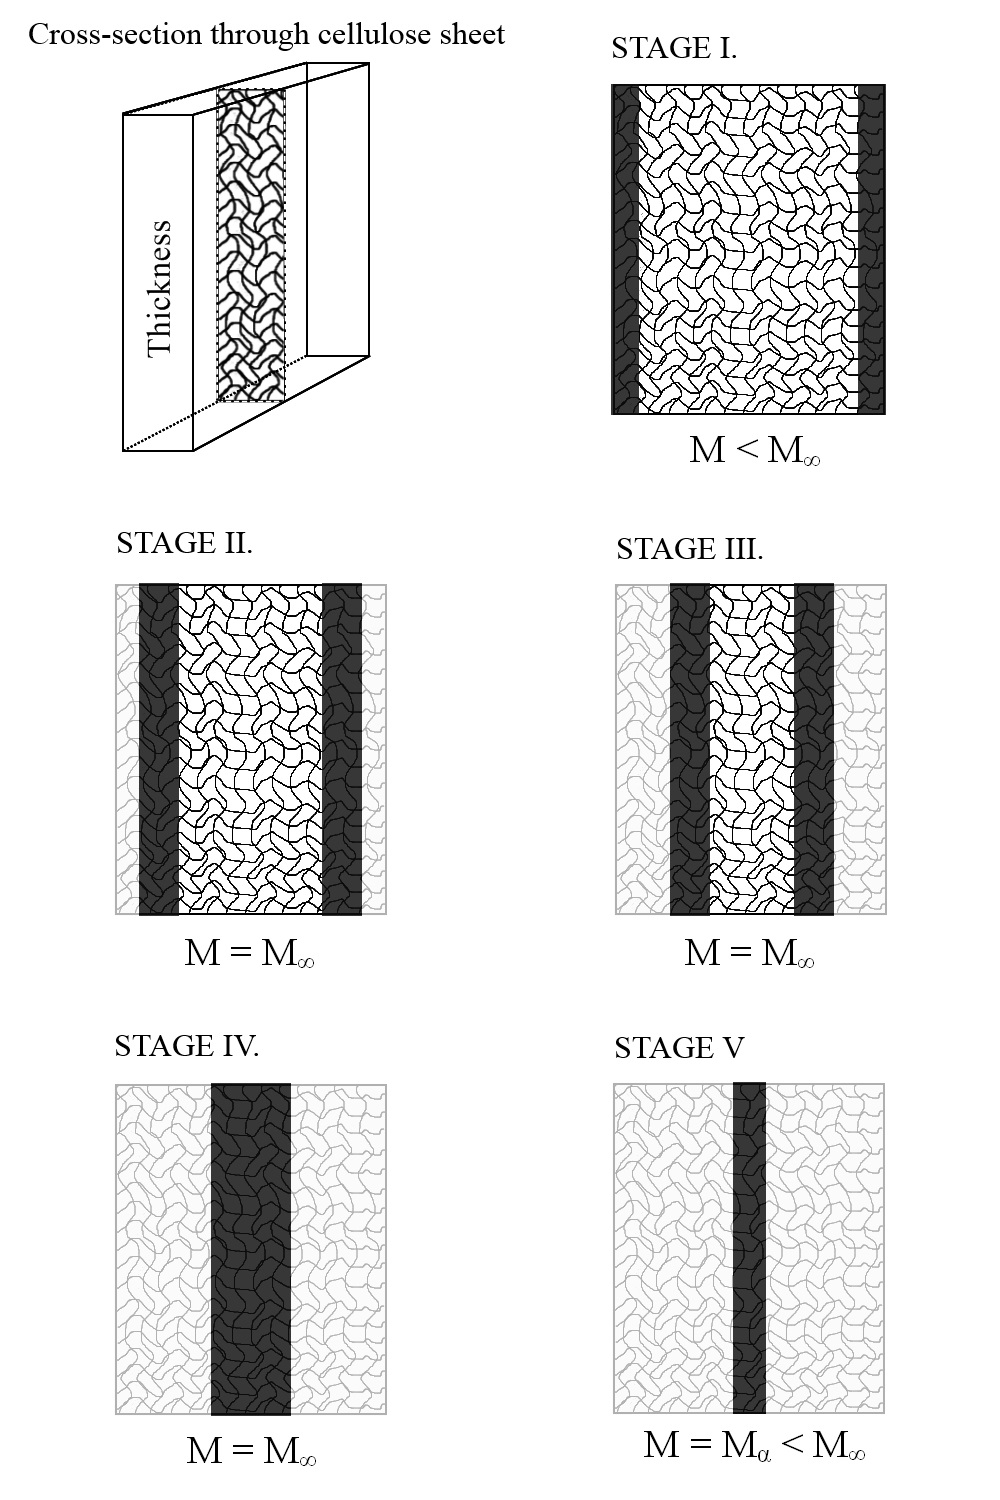
\includegraphics[scale=0.53]{alex_schema.jpg}
  \caption{Conceptual model of cellulolytic biofilm growth and consumption of cellulose sheets. 
    Attachment and growth occures on both sides of the sheet, individual monolayers form on each fiber and result in a band of active biofilm (i.e., the effective sessile biomass) $M$ (dark band). 
    The ideal carrying capacity, $M_{\infty}$, and the actual carrying capacity, $M_{\alpha}$, are explained in \cite{dumitrache2014understanding}.
    Consumed substrate is represented by the light gray areas.
    Figure originally from \cite{dumitrache2015mathematicalModeling}.
  }
  \label{fig:alex_schema}
\end{figure}

A simple mathematical model for celluloltic biofilm activity and growth on model cellulosic substrate was proposed in \cite{dumitrache2014understanding}. 
Here the production of carbon dioxide was used as an indicator of cluture metabolism.
Because of this indicator, they focused on overall biofilm performance rather than on detailed biofilm structure.
The model formed was based on a number of observations on the metabolic acitivity gathered by online carbon dioxide measurements.
For the model formation, attention was also put on high-resolution imaging of different stages of biofilm development \citep{dumitrache2013formFunction} and to the physiological behaviour of substrate modification \citep{dumitrache2013tracking}.

The conceptual model of cellulolytic biofilm growth that was followed for their model is shown in Figure \ref{fig:alex_schema}.
This model is based on the relation between \textit{C. Thermocellum} growth and Whatman cellulose sheet consumption.
The relation is the idea that as the \textit{C. Thermocellum} grows more cellulose sheet is consumed which limites the area of substratum available for bacteria attachment.
Here they express the growth of the biomass in terms of an \textit{ideal} and an \textit{actual} carrying capacity.
The ideal carrying capacity, $M_{\infty}$, refers to the maximum amount of biomass that can be supported when the only limitations are from a deficency of local space.
This value depends on the properties of the substratum and is assumed to be constant since it is independent of the substrate concentration.
The actual carrying capacity, $M_{\alpha}$, references the amount of biomass that can be support when the local concentration of substrate mass is limited.
This value is not constant since it is a function of the current substrate concentration.
In essence, \cite{dumitrache2014understanding} use the carrying capacity as a means to account for the limitations due to spatial effects.

The model developed by \cite{dumitrache2015mathematicalModeling} followed the conceptual five different stages of growth of \textit{C. Thermocellum}.
These five stages were:
\begin{itemize}
  \item Stage I: Independent colonies of cells grow on the matrix of fibers in the substrate. This occurs initially for all the isolated regions of the biofilm.
  \item Stage II: The biofilm grows inwards. The superficial fibres are consumed and newly unsupported biofilms are released from the celluos sheet into the aqueous stream.
  \item Stage III: The active biofilm band stabalizes somewhere around the point where superficial fiber deconstruction rate is the equivalent to the inwards penetration rate of the biofilm.
  \item Stage IV: The progression of the biofilm band continues until the remaining amount of useable substrate becomes limited.
  \item Stage V: The remaining cellulose gets consumed without new biofilm being produced. Instead a new generation of non-adherent cells is formed locally.
\end{itemize}
This formulated a system of ordinary differential equation because of the non-diffusivity of the substrate.
These ordinary differential equations resembled traditional growth models in batch cultures more then the typically complex biofilm model seen in studies \citep{wanner2005mathematical}. %!% find reference for traditional growth models

The model deleveloped in \cite{wang2011spatial} focused more on detailing the spatio-temporal development of a single \textit{C. Thermocellum} biofilm colony.
This was completed by use of a nine-neightbor square cellular automata on a $30 \times 15$ grid with a single grid cell as an innoculation point.
The model results matched the experimental results they gathered.
This was the first model to consider the development of \textit{C. Thermocellum} at a small scale.
Using cellular automata with such a coarse grid gave them a discrete representation of the system they modelled.
In this thesis, one purpose is to extend this concept to a continuous model similar to \cite{eberl2007finite} but instead using assumptions and growth function that match the behaviour of \textit{C. Thermocellum}.

The problem with this is that with \textit{C. Thermocellum} the substratum used for attachment is consumed with biofilm growth.
This, along with the stationary nature of the cellulose sheets, makes this problem significantly different from other biofilm models.
Other biofilm models are based on the aqueous, free-floating environment where biofilms develop.
At the meso-scale, our \textit{C. Thermocellum} system must model the development along the non-diffusing individual fibers of the cellulose sheet structure.
Thus, these two categories of biofilm models differ mainly in their consideration of substrate diffusion, with \textit{C. Thermocellum} there is none.

%!%Look at PDE with Volume filling and compare the model we will use here to the traditional biofilm model.

Our problem originates from the ordinary differential equation model from \cite{dumitrache2015mathematicalModeling}.
Here we include the double-degenerate parabolic model of biofilm formation from \cite{eberl2001deterministic} for the spatial consideration.
This results in a density-dependent diffusion model with reaction terms that match with the behaviour of \textit{C. Thermocellum}.
The spatial operator for biofilm spreading shows two non-standard diffusion effects:
\begin{itemize} 
  \item A power law degeneracy similar to the porous medium equation for local biomass at the interface of the biofilm \cite{gurtin1977diffusion}
  \item A singularity in the diffusion coefficient when the biofilm approaches maximum biomass density. 
\end{itemize}
Both of these effects together lead to the devlopment of sharp and steep interfaces in the model solutions that mark the separation of the actual biofilm from its liquid enviroment.
Such propagating interface problems in partial differiential equations often are difficult to treat numerically.

From a mathematical point of view, \cite{efendiev2002existencelongtime} showed that models which focus on the growth dynamics of biological film are mostly in the form of systems of partial differential equations.
These models take into account some of the significant features of biofilm growth observed throughout the practice.
These features are:
\begin{enumerate}[a)]
  \item the presense of a sharp front of biomass at the solid to fluid transition region,
  \item the existance of a threshold of biomass density,
  \item the spreading of biomass is only notiable when local densities approach the threshold of sustainability,
  \item the use of reaction kinetics mechanisms to model the production of biomass,
  \item the compatibility of biomass spreading with nutrient transfer and consumption mechanism models.
\end{enumerate}
There exist mathematical background for these systems of equation that prove existence and uniqueness of positive and bounded solutions.
However, the complexity of these nonlinear partial differential equations have made practically impossible to provide analytical expressons of the solutions given biologically meaningful initial conditions.
This forces numerical computational approaches to be taken for simulation the growth of these microbial colonies.
Some techniques have been used for these problems in stochastic computational modelling \cite{mccollum2006sorting}.
The finite-difference approach has been proposed in \cite{eberl2001deterministic} for deterministic models.
Differential-discrete cellular automata have been successfully used for the growth of gel beads in \cite{picioreanu1998newCombined}
The finite-element used in \cite{duddu2008combined} and the finite-volume method used in \cite{gallo2003finiteVolume} were both able to handle the complexity of the problem.
The finite-different method was used as an explicit numerical method in \cite{macias-diaz2013efficientNonlinear} for a faster numerical compuation compared to \cite{eberl2001deterministic}.
%!% Haev something here about the semi=implicit method

In this thesis, the finite-difference method is treated as a semi-implicit numerical method similar to \cite{eberl2001deterministic}.
However a new extension is made on this where in a single timestep multiple solutions are found using a fixed-point iteration.
The use of this is that the terms of the system are split into forward difference terms and backwards difference terms.
The forward difference terms are those that make finding an analytic solution difficult.
For each iteration of the fixed-point iteration, the forward difference terms are updated to a new approximation of their \textit{a priori} value.
This turns the semi-implicit method into a fully-implicit method since the next timestep is reached once all the forward difference terms become sufficiently close to their true value for the next timestep.
The validity of this method is unknown and put under scrutiny during this thesis.

